\chapter{In-Hand Manipulation}\label{ch:3-in-hand-manipulation}

The goal of this chapter is to analyze the performance of the reinforcement learning-based manipulation algorithm \gls{dapg}, which employs \gls{il} to constrain the algorithm's search space when solving the relocation task. The relocation task requires the robot hand to pick up an object and move it to a target location.\medskip 

The analysis will focus on the relevant metrics from the training process as well as the final models performance. \medskip

\gls{dapg} was chosen as the algorithm from~\cite{dexmv:-imitation-learning-for-dexterous-manipulation-from-human-videos}, due to it showing the best performance when solving the relocation task. \medskip

Firstly, the \gls{dapg} method is presented and described, followed by the setup for collecting the data used for training. The results are then presented and finally, the findings are discussed and concluded.\medskip

The simulation is done using a \gls{ah}~\cite{learning-complex-dexterous-manipulation-with-deep-reinforcement-learning-and-demonstrations} in the dynamic simulator MuJoCo~\cite{todorov2012mujoco}. The hand is thus equipped with \num{30} controllable parameters, \num{24} for the hand's joints and \num{6} for the hand's position \mvar{\vec{p}_{hnd}=\rvec{p_x,p_y,p_z}} and orientation \mvar{\vec{o}=\rvec{\phi,\theta,\psi}} in \gls{rpy} format. These make up the agent's actions \mvar{a}, while the states {s} also include the position of the prop when performing the relocation task.

\section{Method}\label{sec:3-in-hand-manipulation-method}

\subsection{Demo Augmented Policy Gradient}\label{dapg}

The \gls{dapg} is an approach that expands on the \gls{npg} by introducing a demonstration term to weigh the gradient by \mvar{\lambda_0} and \mvar{\lambda_1}, which are hyperparameters to determine the advantage of state-action pair in demonstrations. \medskip

The parameter update rule to gain \mvar{\theta_{k+1}} can be written as
%
\begin{equation}
    \theta_{k+1} = \theta_k + \sqrt{\frac{\delta}{g^\T F^{-1}_{\theta_k}g}}F^{-1}_{\theta_k}g,
\end{equation}
where \mvar{F_{\theta_k}} is the \gls{fim}, \mvar{g} is the gradient, \mvar{\delta} is the step size, and \mvar{\theta_{k}} is the previous weights.\medskip

The objective function is thus formulated as 
%
\begin{equation}\label{eq:dapg}
    g_{aug} = \sum_{(s,a)\in\rho_{\pi_\theta}}\nabla_\theta \ln \pi_\theta(a|s)A^{\pi_\theta}(s,a) + \sum_{(s,a)\in\rho_{\pi_D}} \nabla_\theta \ln \pi_\theta(a|s) \lambda_0 \lambda_1^k
\end{equation}

Here \mvar{\rho_{\pi_\theta}} is the occupancy measure, which is the probability of ending up in a state action tuple i.e. \mvar{(s,a)}, \mvar{\nabla_\theta} is the derivative operator in terms of \mvar{\theta}, \mvar{\pi_\theta} is the policy under the parameters \mvar{\theta}, \mvar{A^{\pi_\theta}} is the advantage function which tells the advantage gained by performing each action \mvar{\{a_1,a_2,\dots,a_{n_a}\}}, where \mvar{n_a} is the number of actions in the current state, compared to the expected return from taking the currently best action~\cite{advantage-updating}. Finally, \mvar{\rho_{\pi_D}} is the occupancy function from the demonstrations.

\subsection{Data Collection Procedure}
To train \gls{dapg}, raw video data of expert demonstrations of the relocation task is collected. While~\cite{dexmv:-imitation-learning-for-dexterous-manipulation-from-human-videos} provides data for additional tasks i.e. \textit{pour} and \textit{place inside}, these are not of interest in this chapter. The objects used are from the YCB dataset~\cite{ycb} and the demonstrations were recorded by two RGBD cameras.\medskip

The collected data are then parsed to a multi-state pipeline including 3D pose estimation, that being for both the object of interest and the hand and demonstration translation.

\subsubsection{Object Pose Estimation}
The \num{6}-\gls{dof} object poses in the physical setup is found using the PVN3D model, which is a deep learning-based pose estimation model, trained on the YCB data set.\medskip

The \num{6}-\gls{dof} object pose is afterward optimized by minimizing the \gls{PnP} matching error.

\subsubsection{Hand Pose Estimation}

The hand pose is found using the deep learning-based pose estimation model MANO~\cite{mano}, which produces three parameters to represent the hand's pose: \mvar{\theta_t},\mvar{\beta_t} and \mvar{r_t}. \mvar{\theta_t} refers to the 3D rotations of \num{15} joints, \mvar{\beta_t} is the shape
parameters and \mvar{r_t} is the hand root's global pose. These can be combined through hand kinematics to compute the 3D angle of each hand joint
%
\begin{equation}
    \vec{q}^{3d}_t = \mat{J}(\theta_t,\beta_t,r_t)
\end{equation}

By utilizing off-the-shelf skin segmentation techniques such as Combinatorial Color Space Models~\cite{combinatorial-color-space-models-for-skin-detection-in-sub-continental-human-images} and hand detection models on video data, a hand mask \mvar{M_t} is extracted. \mvar{M_t} is overlayed the depth channel of the recorded data and the center of which is the used estimate of \mvar{r_t}. From the video data, the RGB channels are additionally parsed to a MANO which estimates 2D hand joint angles \mvar{\vec{q}_t^{2D}}, along with the hand parameters \mvar{(\theta_t,\beta_t,r_t)}. Having the cameras poses \mat{\Pi} enables the formulation of an optimization problem to determine the optimal \mvar{(\theta_t,\beta_t,r_t)} i.e. \mvar{(\theta_t^\star,\beta_t^\star,r_t^\star)}
%
\begin{equation}
    \theta_t^\star,\beta_t^\star, r_t^\star = \argmin_{\theta_t,\beta_t,r_t} \| \mat{\Pi} \mat{J}(\theta_t,\beta_t, r_t) - \vec{q}_t^{2d} \|^2 + \lambda\| M_t \left( \mat{R}(\theta_t,\beta_t,r_t) - D_t \right) \|^2
\end{equation}
Here \mvar{\lambda=0.001} is a hyperparameter, \mat{R} is a depth rendering function and \mvar{D_t} is the corresponding depth map in frame \mvar{t}.

\subsubsection{Demonstration Translation}

Demonstration translation involves transforming the actions performed by the expert agent with one kinematic structure to a \gls{ml} agent with some other set of actions. This is essential as, while the kinematic structure between the biological human hand and the anthropomorphic robot hand is similar, they are not identical. The similarity can be seen in the hands' kinematic trees in~\appref{app:human-and-robot-hand-kinematics} with their \gls{rom}s in~\appref{app:range-of-motion-shadow-hand} and~\appref{app:range-of-motion-human-hand}.\medskip

This process requires two components: hand motion retargeting and Predicting
robot action. The hand motion retargeting attempts to align the human hand motion to the
robot hand motion, which due to the difference in kinematics is non-trivial as mentioned above. The prediction robot action attempts to estimate the torque necessary for each robot motor to recover the action from only pose estimation results. \medskip

The hand motion retargeting is solved using \gls{tsv}s to describe the optimization problem
\begin{equation}
    \vec{q}^\star_t = \min_{\vec{q}_t} \sum^N_{i=1}\| \vec{v}^{hum}_i(\theta_t,\beta_t,r_t)-\vec{v}^{rob}_i(\vec{q}_t)\|^2+\alpha \| \vec{q}_t - \vec{q}_{t-1} \|^2.
\end{equation}
Here \vec{\vec{v}^{hum}_i(\theta_t,\beta_t,r_t)} computes the \mvar{i}'th \gls{tsv} to the finger tip and middle of the human hand, and the robot's forward kinematics function \mvar{\vec{v}^{rob}_i(\vec{q})} computes the \mvar{i}'th \gls{tsv} to the fingertip and middle of the robot hand. The \gls{tsv}s can be seen illustrated in~\figref{fig:tsv} from the hand root (marked with red) to the finger middle (marked with blue) and tip (marked with green) on the anthropomorphic robot hand.\medskip

\begin{figure}[!h]
	\begin{center}
		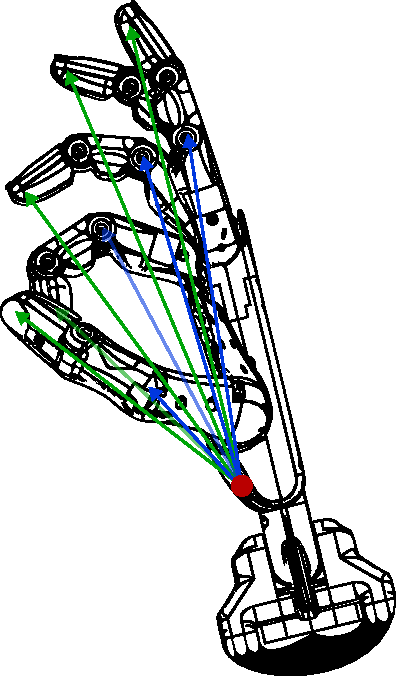
\includegraphics[width=0.3\textwidth]{chapters/3-in-hand-manipulation/fig/tsv.pdf}
	\end{center}
	\caption{The \gls{tsv}s from the hand root (marked with red) to the finger middle (marked with blue) and tip (marked with green) on the anthropomorphic robot hand.}
	\label{fig:tsv}
\end{figure}

The optimization problem was solved using \gls{slsqp} with \mvar{\alpha = 8e-3}.\medskip

The robot action estimation is achieved through the model \mvar{\vec{q}(t)} presented in~\cite{smoothness-maximization-along-a-predefined-path-accurately-predicts-the-speed-profiles-of-complex-arm-movements}, which fulfills the criteria of zero jerk i.e. \mvar{\vec{q}'''(t) \approx 0}. The model enables \mvar{\vec{q}'(t)} and \mvar{\vec{q}''(t)} which through inverse dynamics can be converted to toques \mvar{\vec{\tau}}
\begin{equation}
    \vec{\tau} = f_{inv}\left(\vec{q}(t),\vec{q}'(t),\vec{q}''(t)\right)
\end{equation}
The zero jerk here enables behavior similar to that of a human, which in turn leads to more natural robot motion, as well as ensuring low joint position errors for motors and limiting excessive wear on the physical robot.

\section{Experimental Setup}\label{sec:3-in-hand-manipulation-experimental-setup}

To train and test the \gls{dapg} algorithm, the mug shown in~\figref{fig:manipulation-mug} is chosen as the prop. Additionally, to remain consistent with the original paper~\cite{dexmv:-imitation-learning-for-dexterous-manipulation-from-human-videos} the number of training iterations was \num{2,000} with demonstration hyper parameters \mvar{\lambda_0} and \mvar{\lambda_1} being \num{0.1} and \num{0.99} respectively. Furthermore, the learning rate \mvar{\alpha_{lr}} was set to \num{1.0}, the step size \mvar{\delta} was set to \mvar{0.1} and the discount factor \mvar{\gamma} was \num{0.995}. \medskip

To execute the relocation task, the object is placed on a table and a goal is defined at a random location marked with green silhouette. The experimental setup can be seen in~\figref{fig:experimental-setup-dapg}.

\begin{figure}[!h]
	\centering
	\begin{subfigure}[b]{0.48\textwidth}
		\centering
		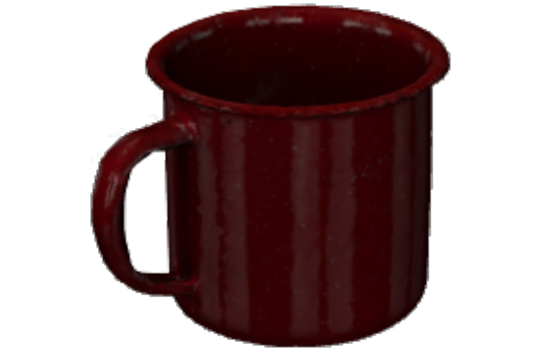
\includegraphics[width=\textwidth]{chapters/3-in-hand-manipulation/fig/mug.pdf}
		\caption{The mug prop from YCB~\cite{ycb} chosen for training.\newline}
		\label{fig:manipulation-mug}
	\end{subfigure}
	\hfill
	\begin{subfigure}[b]{0.48\textwidth}
		\centering
		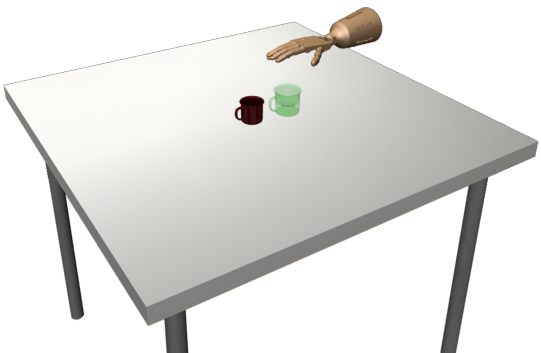
\includegraphics[width=\textwidth]{chapters/3-in-hand-manipulation/fig/experimental-setup-dapg.pdf}
		\caption{The experimental setup used when training the \gls{dapg} algorithm. The figure contains the table platform, the mug prop, the simulated anthropomorphic hand and the goal mug position marked as a green silhouette.}
		\label{fig:experimental-setup-dapg}
	\end{subfigure}
	\caption{The mug prop used for training and the experimental setup.}
	\label{fig:manipulation-mug-experimental-setup-dapg}
\end{figure}

\section{Results}\label{3-in-hand-manipulation-results}
The results gathered from the training procedure are presented here by the 

The running score or cumulative reward obtained by the reinforcement learning agent during training as seen in~\figref{fig:running-score-over-epochs}, The evaluation score or performance of the reinforcement learning agent on a separate set of test episodes or environments as seen in figure~\figref{fig:evaluation-score-over-epochs} and finally the expected return used in policy i.e. the improvement or increase in the surrogate objective function during the policy update as seen in figure~\figref{fig:surrogate-improvements-over-epochs}.

\begin{figure}[!h]
	\begin{center}
		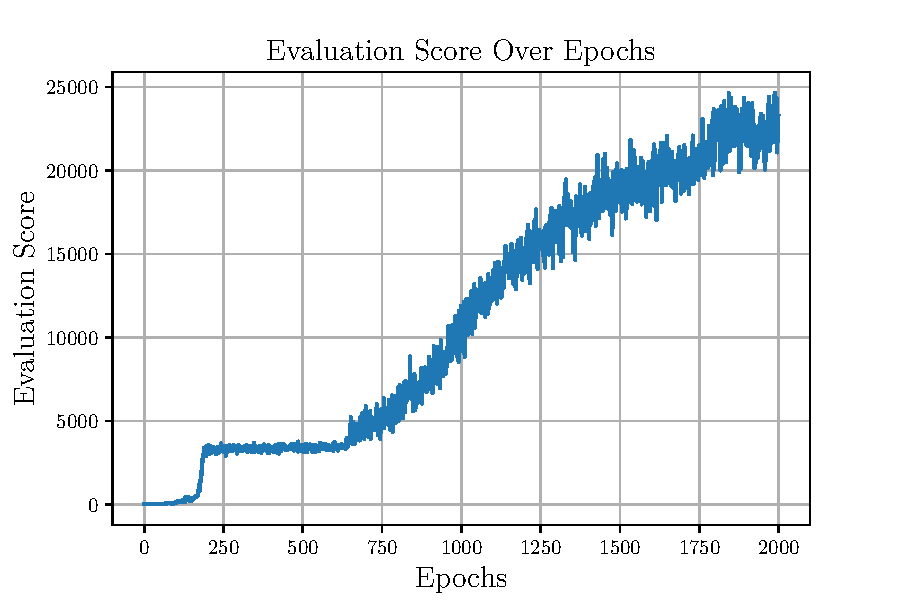
\includegraphics[width=0.8\textwidth]{chapters/3-in-hand-manipulation/fig/evaluation-score-over-epochs.pdf}
	\end{center}
	\caption{The \gls{tsv}s from the hand root (marked with red) to the finger middle (marked with blue) and tip (marked with green) on the anthropomorphic robot hand.}
	\label{fig:evaluation-score-over-epochs}
\end{figure}

\begin{figure}[!h]
	\begin{center}
		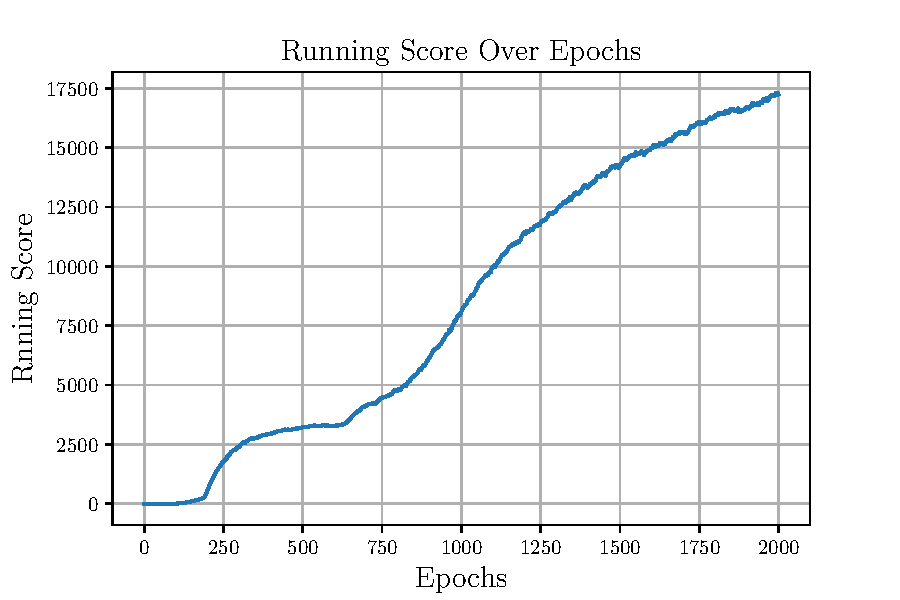
\includegraphics[width=0.8\textwidth]{chapters/3-in-hand-manipulation/fig/running-score-over-epochs.pdf}
	\end{center}
	\caption{The \gls{tsv}s from the hand root (marked with red) to the finger middle (marked with blue) and tip (marked with green) on the anthropomorphic robot hand.}
	\label{fig:running-score-over-epochs}
\end{figure}

\begin{figure}[!h]
	\begin{center}
		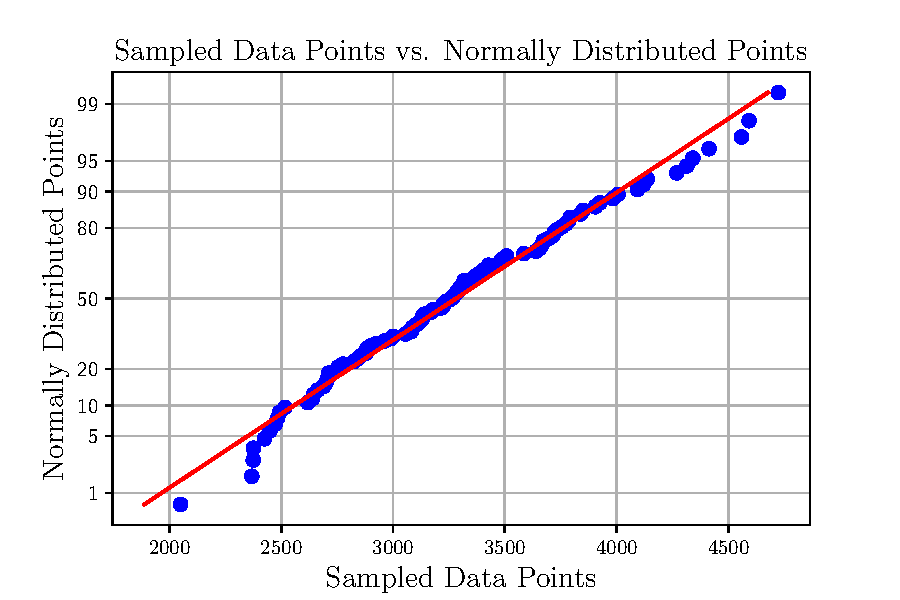
\includegraphics[width=0.8\textwidth]{chapters/3-in-hand-manipulation/fig/surrogate-improvements-over-epochs.pdf}
	\end{center}
	\caption{The \gls{tsv}s from the hand root (marked with red) to the finger middle (marked with blue) and tip (marked with green) on the anthropomorphic robot hand.}
	\label{fig:surrogate-improvements-over-epochs}
\end{figure}

Once trained, the best policy was saved and the reward was sampled over \num{100} iterations, both for the model trained and the one provided by the authors resulting in~\figref{fig:probability-of-getting-a-reward}. 

\begin{figure}[!h]
	\begin{center}
		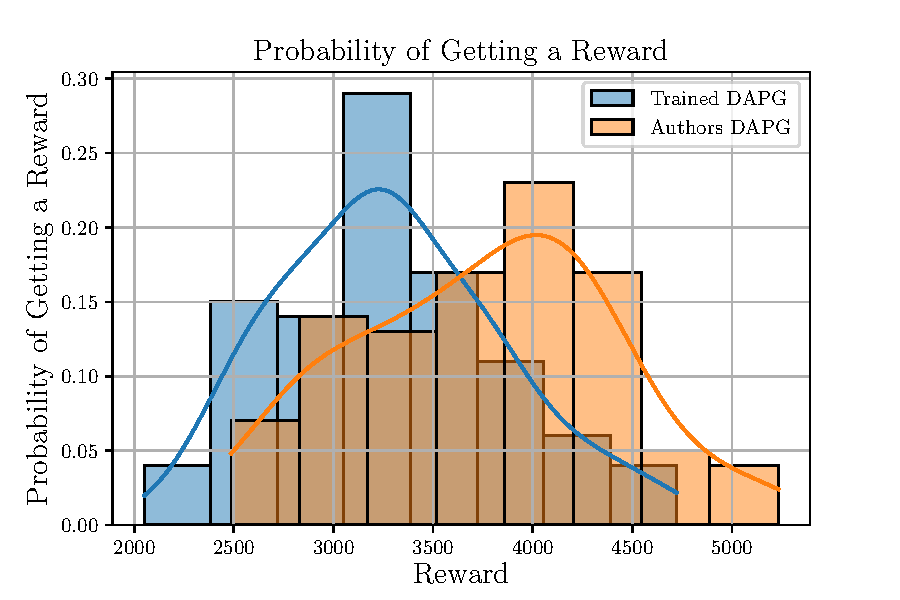
\includegraphics[width=0.8\textwidth]{chapters/3-in-hand-manipulation/fig/probability-of-getting-a-reward.pdf}
	\end{center}
	\caption{The \gls{tsv}s from the hand root (marked with red) to the finger middle (marked with blue) and tip (marked with green) on the anthropomorphic robot hand.}
	\label{fig:probability-of-getting-a-reward}
\end{figure}

To compare the resulting algorithm to the one provided by the authors, it is of interest to test if the reward distributions resulting from experiments come from the same distribution. To determine the normality of each algorithm's performance, normal plots are computed as shown in~\figref{fig:sampled-data-points-vs-normally-distributed-points-authors}. From these plots, normality is assumed.

\begin{figure}[!h]
	\centering
	\begin{subfigure}[b]{0.48\textwidth}
		\centering
		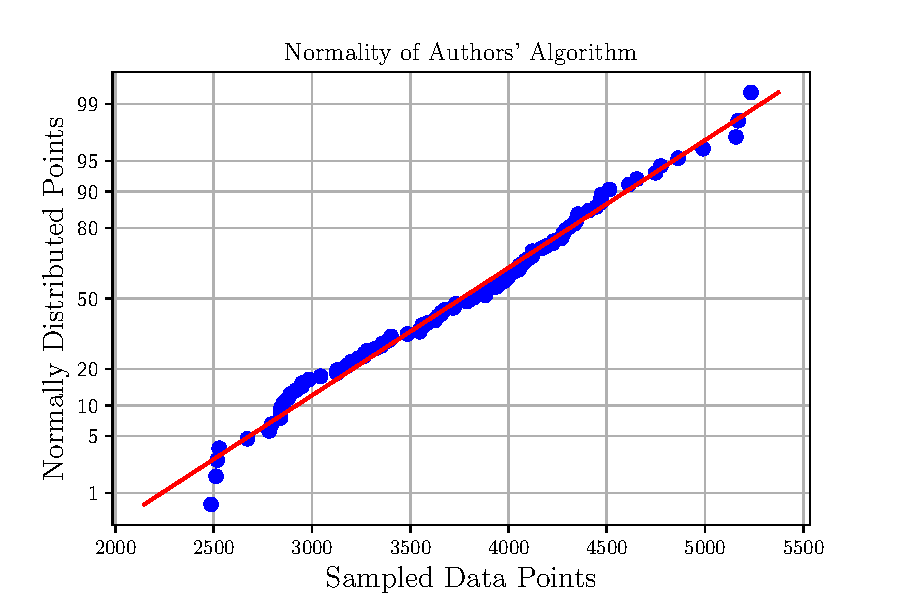
\includegraphics[width=\textwidth]{chapters/3-in-hand-manipulation/fig/sampled-data-points-vs-normally-distributed-points-authors.pdf}
		\caption{test}
		\label{fig:sampled-data-points-vs-normally-distributed-points-authors}
	\end{subfigure}
	\hfill
	\begin{subfigure}[b]{0.48\textwidth}
		\centering
		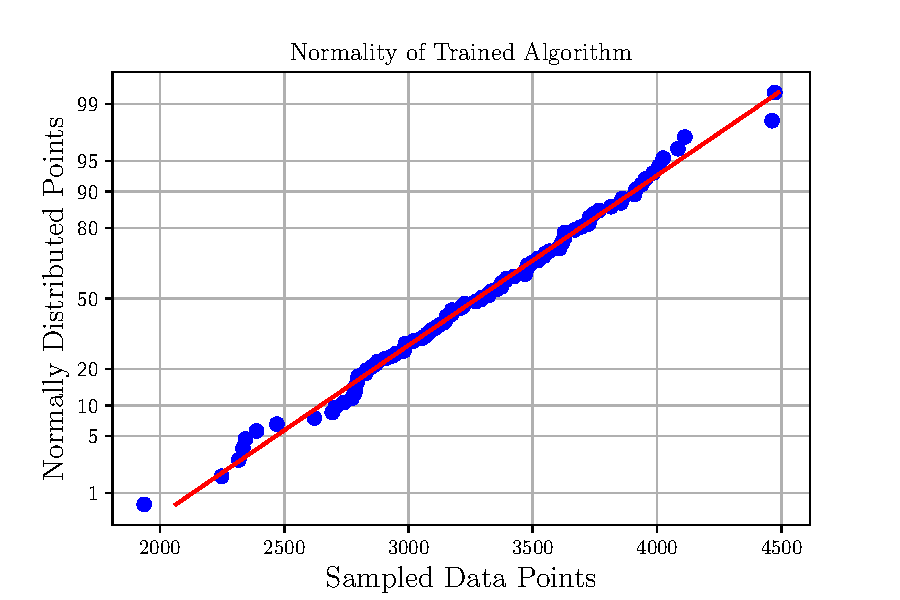
\includegraphics[width=\textwidth]{chapters/3-in-hand-manipulation/fig/sampled-data-points-vs-normally-distributed-points-trained.pdf}
		\caption{test}
		\label{fig:sampled-data-points-vs-normally-distributed-points-trained}
	\end{subfigure}
	\caption{The mug prop used for training and the experimental setup.}
	\label{fig:sampled-data-points-vs-normally-distributed-points-trained-authors}
\end{figure}

when testing for homoscedasticity the Bartlett test is applied, resulting in the p-value \mvar{p_{bart}\approx 0.0044}. Due to the common threshold for rejecting homoscedasticity being \num{0.05}, which is considered sufficiently close to \num{0.0044}, both parametric and non-parametric \gls{anova} i.e. One-Way \gls{anova} and Kruskal-Wallis tests are applied. \medskip

The One-Way \gls{anova} resulted in a p-value of \mvar{p_{\text{ANOVA}}\approx 1.13\cdot 10^{-8}}, while Kruskal-Wallis resulted in \mvar{p_{\text{KW}}\approx 6.85\cdot 10^{-8}}.

A demonstration can be seen illustrated in~\figref{fig:ai-frames}

\begin{figure}[!h]
	\centering
	\begin{subfigure}[b]{0.32\textwidth}
		\centering
		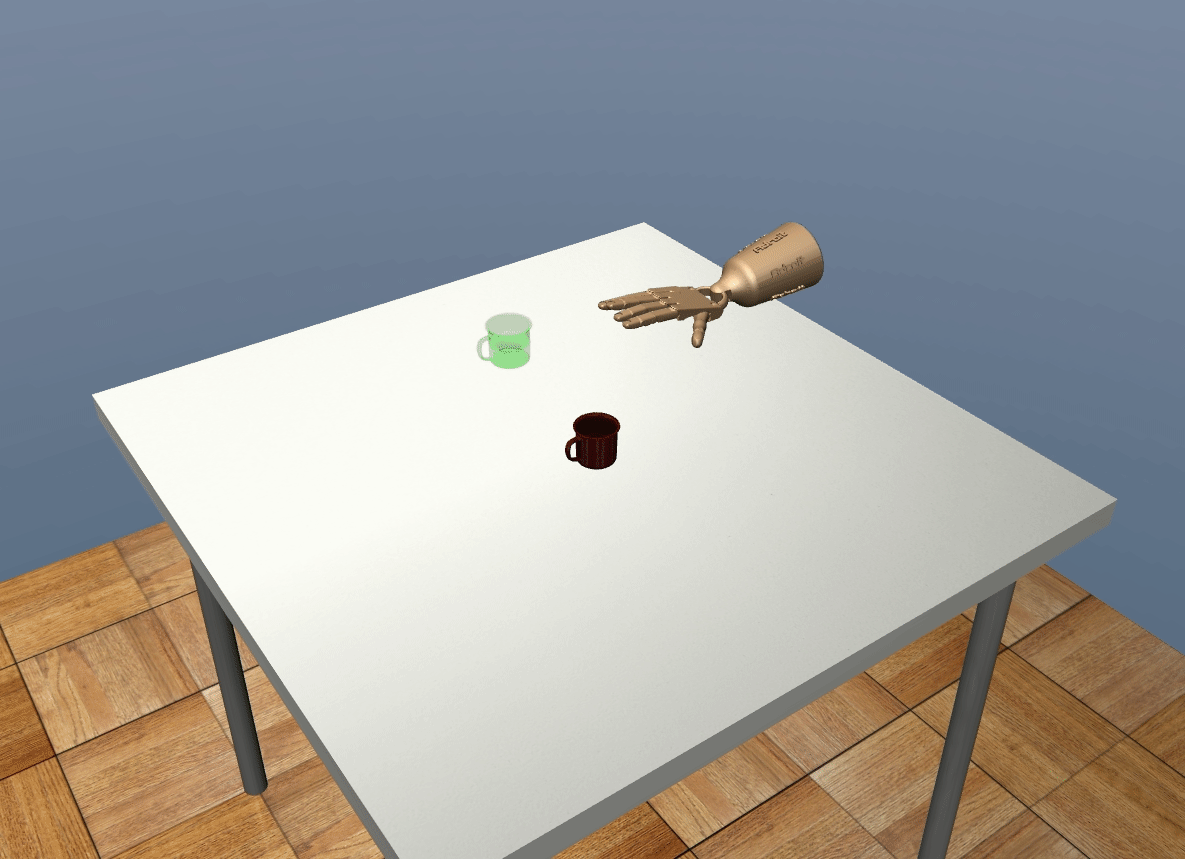
\includegraphics[width=\textwidth]{chapters/3-in-hand-manipulation/fig/frame_10.png}
		\caption{Finger in contact with a flat surface.}
		\label{fig:ai-frame-1}
	\end{subfigure}
	\hfill
	\begin{subfigure}[b]{0.32\textwidth}
		\centering
		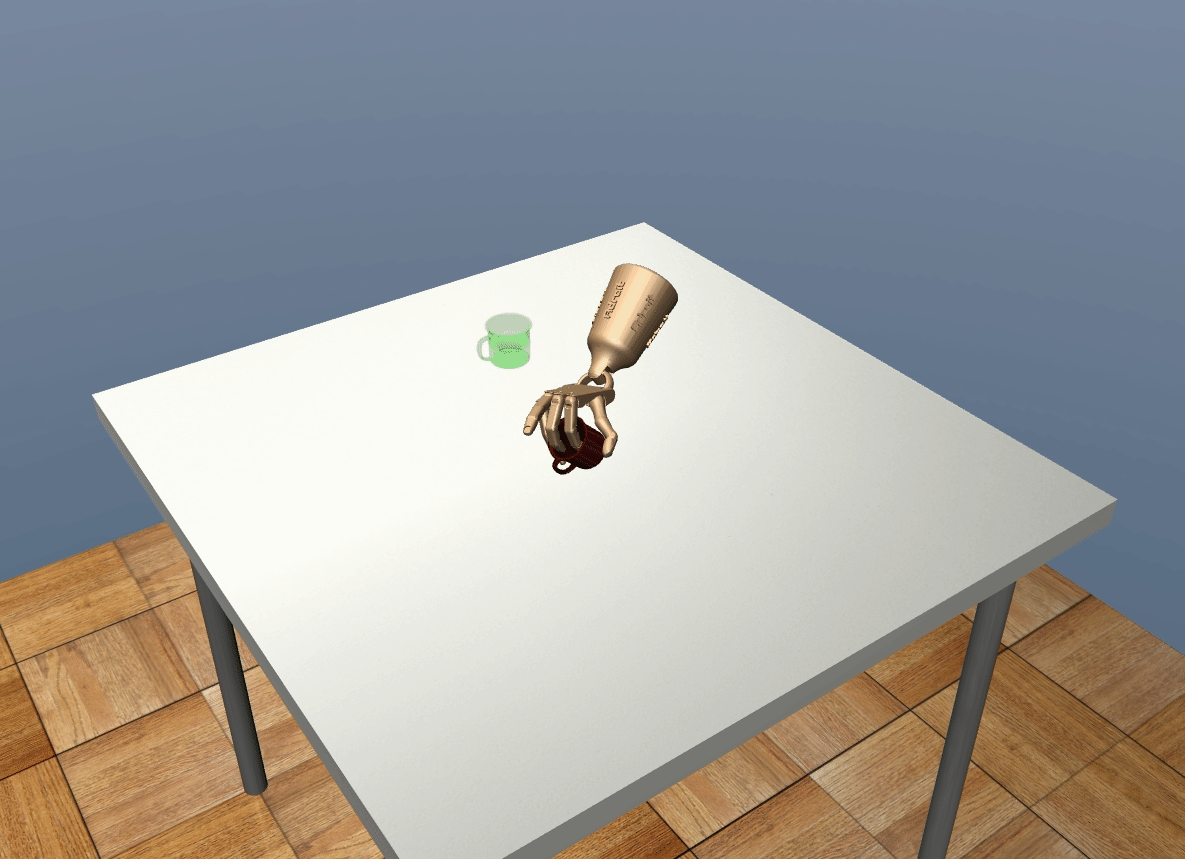
\includegraphics[width=\textwidth]{chapters/3-in-hand-manipulation/fig/frame_21.png}
		\caption{Finger in contact with an edge.}
		\label{fig:ai-frame-2}
	\end{subfigure}
	\hfill
	\begin{subfigure}[b]{0.32\textwidth}
		\centering
		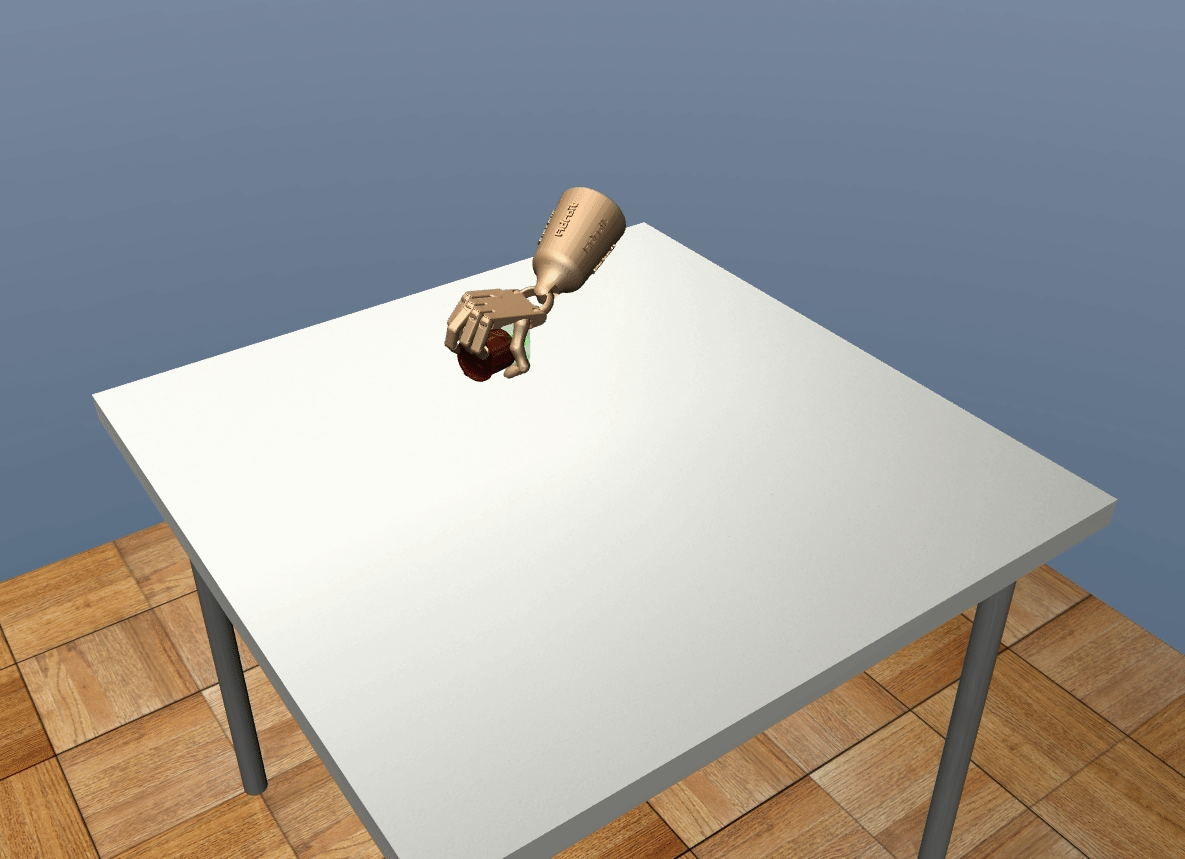
\includegraphics[width=\textwidth]{chapters/3-in-hand-manipulation/fig/frame_44.png}
		\caption{Finger in contact with a smooth surface.}
		\label{fig:ai-frame-3}
	\end{subfigure}
		\caption{The four surfaces used to test the performance of the \gls{dl} model's ability to represent surfaces.}
		\label{fig:ai-frames}
\end{figure}

\newpage
\section{Discussion \& Conclusion}

% This chapter has shown that the \gls{dapg} successfully learn from demonstration and can perform the dexterous manipulation task of relocation. The results from the trained algorithm appear normally distributed but do not strictly fulfill homoscedasticity. Further investigation showed a statistically significant difference between the two underlying distributions, indicating a better performance from the agent trained by the authors.

The findings of this chapter provide strong evidence that the \gls{dapg} algorithm successfully learns from demonstrations and demonstrates its capability to perform the dexterous manipulation task of relocation. The trained algorithm exhibits promising results, with outcomes that follow a distribution resembling a normal distribution.\medskip

However, upon closer analysis, it becomes apparent that the distribution of the algorithm's performance does not strictly adhere to the assumption of homoscedasticity. Homoscedasticity assumes that the variances of the performance values are equal across the distribution. In this case, the observed departure from homoscedasticity suggests the presence of variability or heterogeneity in the algorithm's performance across different relocation tasks. \medskip

To gain further insights, additional investigation was conducted to compare the underlying distributions. The results of this investigation revealed a statistically significant difference between the distributions associated with the agent trained by the authors and the alternative distributions. This significant difference implies that the agent trained by the authors outperforms the alternatives in terms of its ability to successfully accomplish the relocation task.\medskip

In summary, the chapter highlights the successful learning capabilities of the \gls{dapg} algorithm from demonstrations, specifically in the context of the dexterous manipulation task of relocation. The outcomes generated by the trained algorithm exhibit a distribution that resembles a normal distribution, although it deviates from strict homoscedasticity. By conducting further analysis and comparing underlying distributions, it was determined that the agent trained by the authors performs significantly better than the alternative approaches. These findings underscore the effectiveness and superior performance of the agent trained using the \gls{dapg} algorithm in tackling the challenging relocation task.